\subsection{Bilanzräume in der Energiewirtschaft}

%%%%%%%%%%%%%%%%%%%%%%%%%%%%%%%%%%%%%%%%%%%%%%%%%%%%%%%%%%%%%%%%%%%%%%%%%%%%%%%%%%%%%%%%%%%%%%%%%%%%%%%%%%%%%%%%%%%%%%%%%%%%%%%%%%%%%%%%%%%%%%%%%%%%%%%%%%%%%%%%%%%

\subsubsection{Bilanzraumgrenzen zur Abbildung des bilanzierten Systems}
Eine Bilanz bezieht sich gemäß Ahrendts (2014, Kapitel 1.5) auf das von der Systemgrenze eingeschlossene Kontrollgebiet. 
Die Systemgrenze kann dabei unter Berücksichtigung der Zweckmäßigkeit frei definiert werden (\cite[Kapitel 1.5]{Ahrendts.2014}).
Das definierte System kann auch als Bilanzraum bezeichnet werden, da die Berechnung der in einen Bilanzraum ein- und austretenden Ströme als Bilanzierung bezeichnet wird (\cite[S. 65]{Rönsch.2015}).
Einen Ansatz zur Definition von Bilanzräumen liefert Miller (2016, S. 105) mit der Konkretisierung von Bewertungsräumen mittels Kriterien der Bilanzgrenze, dem 
Aggregationsniveau und der Bewertungseinheit. Das definierte System Dient der Bewertung der Nutzung der Ressourcen wobei der Effizienzbegriff eine zentrale Rolle spielt (\cite[S. 107]{Miller.2016}).
Miller (2016, S. 107) definiert die Effizienz nach Gleichung \eqref{EffizienzgleichungMiller}.

\begin{equation}
    \text{Effizienz} := \frac{\text{Erreichter Nutzen}}{\text{Aufwand}}
    \label{EffizienzgleichungMiller}
\end{equation}

Der Aufwand umfasst nach Miller (2016, S. 108f.) unterschiedliche Ressourcen, wobei im Kontext energiewirtschaftlicher Fragestellungen der Fokus auf der Ressource Energie 
liegt.
Der Nutzen ist vom Untersuchungsgegenstand abhängig und wird im Kontext der energiewirtschaftlichen 
Fragestellung häufig über Energiedienstleitstungen operationalisiert (\cite[S. 107]{Miller.2016}). Betrachtet man dass der Nutzen grundsätzlich durch Befriedigung 
von Bedürfnissen beschrieben wird entsteht im Kontext der Energiewirtschaft ein Nutzenergiebedarf zur Befriedigung der Bedürfnisse im Rahmen einer Energiedienstleitstung 
(\cite[S. 107]{Miller.2016}). 
Sowohl die Ressourcen des Aufwands als auch die Energiedienstleistung auf Nutzenseite werden durch eine Bewertungseinheit formalisiert (\cite{Miller.2016}).
Der Nutzen wird meist implizit durch den gewählten Untersuchungsgegenstand definiert (\cite[S. 110]{Miller.2016}).
Die in \eqref{EffizienzgleichungMiller} aufgestellte Nutzen-Aufwand Relation stellt die Grundlage der Definition der Bilanzraumgrenze dar. 
Die Bilanzraumgrenze lässt sich somit in die Aufwandsseitige Bilanzgrenze, die alle zu bilanzierenden Ressourcen umfasst und die Nutzenseitige Bilanzrgrenze die sich auf 
die zu Bilanzierende Energiedienstleitstung bezieht (\cite[S. 111]{Miller.2016}).  

Das von Miller (2016) beschriebene Konzept bringt eine neue Perspektive auf die in \eqref{BilanzierungsgleichungAhrendt} und \eqref{BilanzierungsgleichungAhrendtStrom} 
aufgestellte Bilanzgleichung. Sie bringt das Prinzip der Effizienz ein und teilt eine Bilanz in Aufwands und Nutzenseite. 
Aufwandsseitig sind die in \eqref{BilanzierungsgleichungAhrendt} zufließenden Ströme, also die dem System zugeführten Ressourcen der Zustandsgröße zu betrachten. 
Nutzenseitig müssen abfließende Ströme, also die aus dem System fließende Energie zur Befriedigung der Energiedienstleistung der Zustandsgröße betrachtet werden. 
Die abfließenden Ströme werden nach Energiedienstleistung mit Nutzengrößen operationalisiert (\cite{Miller.2016}).

%%%%%%%%%%%%%%%%%%%%%%%%%%%%%%%%%%%%%%%%%%%%%%%%%%%%%%%%%%%%%%%%%%%%%%%%%%%%%%%%%%%%%%%%%%%%%%%%%%%%%%%%%%%%%%%%%%%%%%%%%%%%%%%%%%%%%%%%%%%%%%%%%%%%%%%%%%%%%%%%%%%

\subsubsection{Zustandsgrößen, Nutzengrößen und Nutzenergiebedarf}
In einem Thermodynamischen System wird der augenblickliche Zustand durch die Zustandsgrößen beschrieben, wobei diese in intensive und extensive Zustandsgrößen 
unterschieden werden (\cite[S. 66]{Konstantin.2023}). Die innere Energie U ist eine extensive Zustandsgröße (\cite[S. 65]{Konstantin.2023}), und rückt in den 
Fokus da es sich um eine energetische Zustandsgröße handelt. Das Verhalten einer Zustandsgröße ist in \eqref{BilanzierungsgleichungAhrendt} und \eqref{BilanzierungsgleichungAhrendtStrom} 
beschrieben.

In dieser Forschung bezieht sich der Untersuchungsgegenstand aufgrund der verortung der Organisationen im tetriären Wirtschaftssektors auf Gebäudeenergie. 
Es müssen also auf der Grundlage dieses Untersuchungsgegenstands angemessene Nutzengrößen mit entsprechenden Bewertungseinheiten erfasst werden. 
Da auch die Definition der Systemgrenze vom Untersuchungsgegenstand beeinflusst wird (\cite[S. 109]{Miller.2016}) gilt die Zweckmäßigkeit der Systemgrenze 
auch für die zu untersuchenden Nutzengrößen.
Die DIN EN ISO 50001:2018-12 gibt mit dem Ziel der fortlaufenden Verbesserung der energiebezogenen Leistung eine Vorgabe zur zweckmäßigen Definition der Nutzengröße 
(\cite[S. 11]{DIN50001.2018}).
Die Vornorm DIN V 18599-1:2018-09, herausgegeben vom Deutschen Institut für Normung e. V. (2018, S. 1), behandelt die energetische Bewertung von Gebäuden und stellt ein 
Verfahren zur Durchführung der Gesamtenergiebilanz bereit (\cite[S. 9]{DIN18599.2018}). Ihre Ausrichtung auf die energetische Bewertung erfüllt die Zweckmäßigkeit der 
DIN EN ISO 50001:2018-12. Der Fokus auf die Bewertung von Gebäuden entspricht der Zielsetzung der DIN V 18599-1:2018-09. 

Im Rahmen der energetischen bewertung von Gebäuden betrachtet die DIN V 18599-1:2018-09 die Bilanzierung des Nutz-, End- und Primärenergiebedarf (\cite{DIN18599.2018}).
In einem energiewirtschaftlichen Rahmen hat besonders der Nutzeenergiebedarf eine Große Bedeutung da er aus der Befriedigung der Bedürfnisse im Rahmen einer 
Energiedienstleistung resultiert (\cite[S. 107]{Miller.2016}).

\begin{figure}[H]
    \centering
    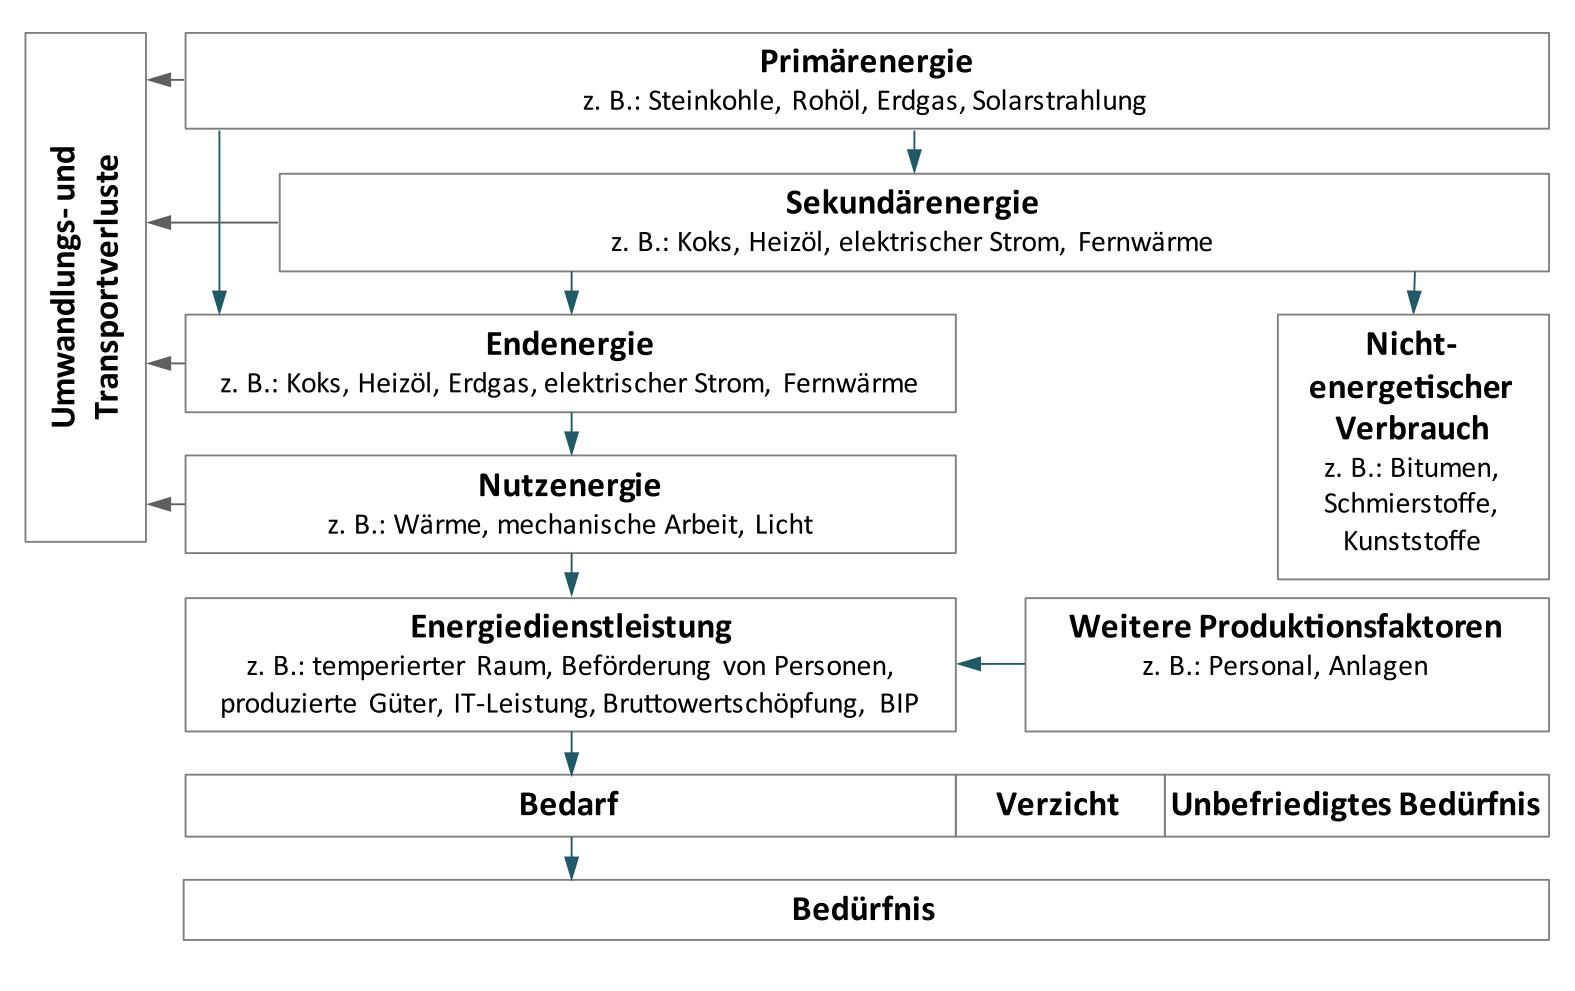
\includegraphics[width=0.8\textwidth]{../../Ressourcen/Abbildungen/Energiefluss_Miller.jpg}
    \caption{Energieflussschema. (Dargestellt von Miller (2016))}
    \label{fig:Energieflussschema_Miller}
\end{figure}

Im Energieflussdiagramm \eqref{fig:Energieflussschema_Miller} wird die Nutzenergie zwischen der Endenergie und der Energiedienstleistungen verortet. 
Da die Endenergie die Energiemenge ist, die dem Bilanzraum zur bestimmungsgemäßen Nutzung bereitgestellt wird (\cite[Kapitel 3.1.2]{DIN18599.2018}), 
Repräsentiert diese Energieform die Menge der potentiellen Ressourcen auf Aufwandsseite der Bilanzierung.
Außerdem wird der praktische Sachverhalt veranschaulicht dass bei der Umwandlung von Endenergie in Energiedienstleistungen über die Nutzenergie 
Umwandlungs und Transportverluste berücksichtigt werden müssen.

Die DIN V 18599-1:2018-09 definiert die Heizung, Kühlung, Lüftung, Trinkwarmwasseraufbereitung und Beleuchtung von Gebäuden oder Gebäudezonen 
als relevante Nutzengrößen zur energetischen Bewertung von Gebäuden (\cite{DIN18599.2018}). 
Somit wird im von Miller (2016) aufgestellten Konzept der Nutzenergiebedarf der jeweiligen Nutzengröße durch die Nutzenergie gedeckt, 
und muss je nach Nutzengröße unterschiedlich definiert werden. Die Nutzenergie wird im Konzept von Miller (2016) durch die Ressourcen repräsentiert.
Im Rahmen der Vornorm wird der Nutzenergiebedarf als Überbegriff für Nutzwärmebedarf, Nutzkältebedarf, Nutzenergiebedarf für Tinkwarmwasser, Beleuchtung und 
Befeuchtung definiert (\cite[Kapitel 3.1.3]{DIN18599.2018}).
Der Nutzenergiebedarf der Beleuchtung ist definiert als rechnerisch ermittelter Energiebedarf, der sich ergibt, wenn die Gebäudezone mit der im Nutzungsprofil 
festgelegten Beleuchtungsqualität beleuchtet wird (\cite[Kapitel 3.1.6]{DIN18599.2018}). 
Analog dazu versteht sich die Nutzeenergie für die Beleuchtung als die Energiemenge die zur Ausreichenden Beleuchtung der Gebäudezone aufgewendet werden muss (\cite[Kapitel 5.3.1]{DIN18599.2018}).
Der Nutzwärmebedarf hingegen ist der rechnerisch ermittelter Wärmebedarf, der zur Aufrechterhaltung der festgelegten thermischen Raumkonditionen innerhalb einer Gebäudezone während der Heizzeit benötigt wird
rechnerisch ermittelter Energiebedarf, der sich ergibt, wenn die Gebäudezone mit der im Nutzungsprofil festgelegten Beleuchtungsqualität beleuchtet wird(\cite[Kapitel 3.1.4]{DIN18599.2018}).
Der Nutzkältebedarf ist der rechnerisch ermittelter Kühlbedarf, der zur Aufrechterhaltung der festgelegten thermischen Raumkonditionen innerhalb einer Gebäudezone benötigt wird in Zeiten, 
in denen die Wärmequellen eine höhere Energiemenge anbieten als benötigt wird(\cite[Kapitel 3.1.5]{DIN18599.2018}).
Die Wärmeenergie ist die Wämemenge, die der Gebäudezone zusätzlich (bedarfs-)geregelt zugeführt werden muss, um die vorgegebene 
Sollinnentemperatur einzuhalten (\cite[Kapitel 5.3.1]{DIN18599.2018}).
Der Nutzenergiebedarf für die Trinkwarmwasserbereitung ist definiert als der rechnerisch ermittelte Kühlbedarf, der zur Aufrechterhaltung der festgelegten thermischen Raumkonditionen innerhalb einer Gebäudezone benötigt wird in Zeiten, in denen die Wärmequellen eine höhere Energiemenge anbieten als benötigt wird
rechnerisch ermittelter Energiebedarf, der sich ergibt, wenn die Gebäudezone mit der im Nutzungsprofil festgelegten Menge an Trinkwarmwasser entsprechender Zulauftemperatur versorgt wird (\cite[Kapitel 3.1.7]{DIN18599.2018}).
Die Nutzenergie für die Trinkwarmwasserbereitung bedeutet die Energiemenge für die Erwärmung des Trinkwassers von der Kaltwassertemperatur auf die 
Warmwassertemperatur an der Entnahmestelle (\cite[Kapitel 5.3.1]{DIN18599.2018}).
Im Rahmen der Luftaufbereitung versteht sich die Nutzenergie als Energiemenge die zum Erwärmen, Kühlen, Befeuchten und Entfeuchten der Luft in einer 
raumlufttechnischen Anlage zu- beziehungsweise abgeführt werden muss um den erforderlichen Zuluftzustand zu erreichen (\cite[Kapitel 5.3.1]{DIN18599.2018}).

Abbildung \eqref{fig:Übersicht_Bilanzräume} Ordnet den mithilfe der DIN V 18599-1:2018-09 erfassten Untersuchungsgegenstand in das von Miller (2016) erarbeitete Konzept der 
Bewertungsräume ein.

\begin{figure}[H]
    \centering
    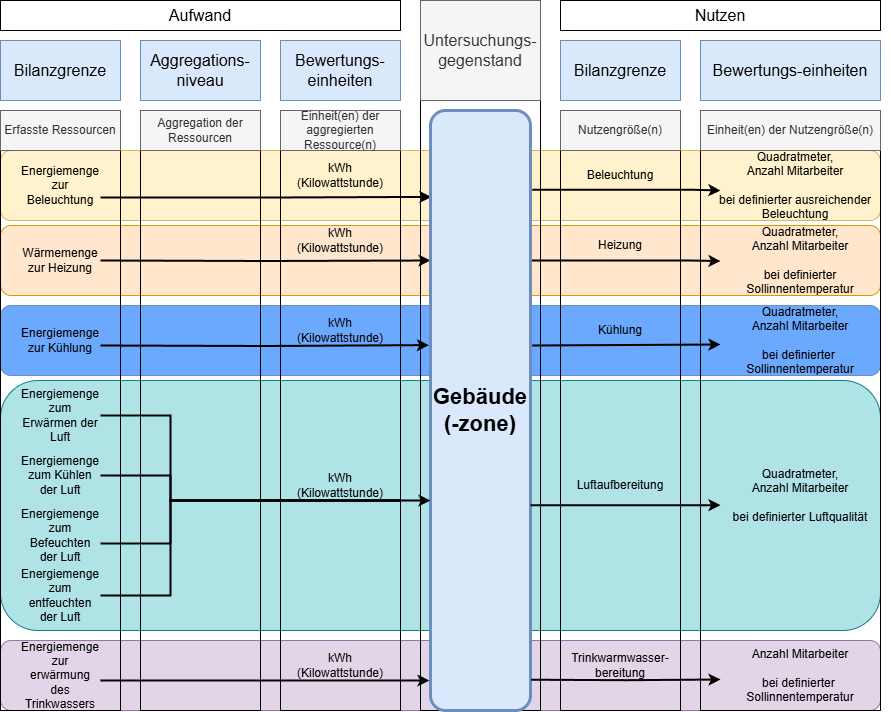
\includegraphics[width=1\textwidth]{../../Ressourcen/Abbildungen/Nutzengröße_Bewertungseinheit.png}
    \caption{Übersicht Bilanzräume. (Eigene Darstellung basierend auf Miller (2016) und DIN V 18599-1:2018-09 (2018))}
    \label{fig:Übersicht_Bilanzräume}
\end{figure}

%%%%%%%%%%%%%%%%%%%%%%%%%%%%%%%%%%%%%%%%%%%%%%%%%%%%%%%%%%%%%%%%%%%%%%%%%%%%%%%%%%%%%%%%%%%%%%%%%%%%%%%%%%%%%%%%%%%%%%%%%%%%%%%%%%%%%%%%%%%%%%%%%%%%%%%%%%%%%%%%%%%

\subsubsection{Energieströme und Bewertungseinheiten}
In der Gleichung \eqref{BilanzierungsgleichungAhrendtStrom} wird der Strom einer Zustandsgröße als Menge der Zustandsgröße in einem infinitesimal kleinen Zeit-
intervall definiert, welches im Grenzwert gegen 0 geht. Folglich wird ein Strom von Ahrendts (2014) als Menge einer Zustandsgröße zu einem bestimmten Zeitpunkt 
definiert. 

In Gleichung \eqref{BilanzierungsgleichungAhrendt} wird zwischen in das System zu- und abfließende Ströme der Zustandsgröße Unterschieden.
Die zufließenden Ströme können als Ressourcen der Aufwandsseite im von Miller (2016) aufgestellten Konzept der Bewertungsräume betrachtet werden, 
wobei energetische Ressourcen im Vordergrund stehen. Aufwandsseitige Ressourcen können zu einer Ressource mit einer Bewertungseinheit 
zusammengefasst werden (\cite[S. 112]{Miller.2016}). Sollten nach erfassung und optionaler aggregation der Ressourcen mehrere Ressourcenkategorien bestehen, 
können diese mit unterschiedlichen Bewertungseinheiten bilanziert werden (\cite[S. 112]{Miller.2016}). Im Rahmen dieser Forschungsarbeit werden 
Aufwandsseitig jedoch ausschließlich Energieressourcen betrachtet.
Sie Stammen somit aus dem Bereich der Endenergie und haben die Bewertungseinheit: kWh und deren Vielfaches da diese Einheit bei Energiebilanzen in der Regel für alle 
Energieformen bevorzugt verwendet wird (\cite[S. 65]{Konstantin.2023}).

Die abfließenden Ströme in \eqref{BilanzierungsgleichungAhrendt} repräsentieren die Nutzenseite des von Miller (2016) aufgestellten Konzepts.
Um die Nutzenseite abzubilden ist eine Konkretisierung der Energiedienstleistung durch eine angemessene Bewertungseinheit, 
welche vom Untersuchungsgegenstände impliziert wird notwendig (\cite{Miller.2016}). Diese Bewertungseinheit ist keine Energieeinheit, und 
kann beispielsweise bei der Untersuchung der Temperierung von Räumen die Quadratmeteranzahl des Bilanzraums bei einer definierten 
soll Temperierung sein (\cite{Miller.2016}). 

Eine praktische Herausforderung im Rahmen der Bilanzierung ist die Energiedatensammlung der zu erfassenden Ströme zu der auch die DIN EN ISO 50001:2018-12 vorgaben macht. 
Die DIN EN ISO 50001:2018-12 (2018, Kapitel 6.6, A.6.6) stellt Anforderungen und Qualitätskriterien an die Datensammlung in Organisationen.
Diese verpflichtet Organisationen dazu Hauptmerkmale ihrer Tätigkeiten, die sich auf die energiebezogene Leistung auswirken zu identifizieren, und diese in geplanten 
Zeitabständen zu messen, überwachen und analysieren (\cite[S. 23]{DIN50001.2018}).
Teil der zu erfassenden Hauptmerkmale sind relevante Variablen bezüglich wesentlicher Energieeinsätze, den Energieverbrauch bezüglich wesentlicher Einsätze 
und der Organisation und betriebliche Kriterien bezüglich wesentlicher Energieeinsätze(\cite[S. 23]{DIN50001.2018}).
Die komplexität der Umsetzung ist dabei nicht vorgeschrieben und kann von einfachen Zählwerten bis hin zu umfangreichen Werten aus Überwachungs- und Messystemen mit 
Softwareandwendung reichen (\cite[S. 36]{DIN50001.2018}).

%%%%%%%%%%%%%%%%%%%%%%%%%%%%%%%%%%%%%%%%%%%%%%%%%%%%%%%%%%%%%%%%%%%%%%%%%%%%%%%%%%%%%%%%%%%%%%%%%%%%%%%%%%%%%%%%%%%%%%%%%%%%%%%%%%%%%%%%%%%%%%%%%%%%%%%%%%%%%%%%%%%

\subsubsection{Energiequellen und -senken}
Gleichung \eqref{BilanzierungsgleichungAhrendt} unterscheidet zwischen Quellen, Senken und zu- beziehungsweise abfließenden Strömen der Zustandsgröße. 
Quell- und Senkenströme treten in einer Energiebilanz nach dem ersten Hauptsatz der Thermodynamik nicht auf da Energie als Erhaltungsgröße ist (\cite[S. 14]{Ahrendts.2014}). 
Im Rahmen der DIN EN ISO 50001:2018-12 bezieht sich der Begriff Energie auf verschiedene Arten von Energie die erworben, gespeichert, aufbereitet, in einer Einrichtung oder einem Prozess verwendet 
oder zurückgewonnen werden können (\cite[Kapitel 3.5.1]{DIN50001.2018}). Energie kann im Rahmen der Norm als Elektrizität, Brennstoff, Dampf, Wärme, Druckluft oder vergleichbares Medium auftreten 
(\cite[Kapitel 3.5.1]{DIN50001.2018}).
Folglich werden alle Energieströme, in denen Energie in eine Energieform umgewandelt wird, die nicht die genannten Kirterien erfüllen als Energiesenken betrachtet. 
Analog dazu werden alle Energieströme, bei denen Energie, die nicht den von der Norm aufgestellten Kriterien entspricht, in eine nach ISO 50001 definierte Energieform 
umgewandelt wird, als Energiequellen betrachtet.
In der Praxis stellen die in Abbildung \eqref{fig:Energieflussschema_Miller} dargestellten Umwandlungs- und Transportverluste Energiesenken dar. Energiequellen können beispielsweise 
PV-Anlagen sein, da diese die Energie des Sonnenlichts, welche nach Definition der DIN EN ISO 50001:2018-12 nicht Nutzbar ist in nutzbare Energie umwandelt und als 
Endenergie zur Verfügung steht.

\subsubsection{Bilanzraumstrukturen}
Bisher wurde die strukturelle Definition von Bilanzräumen unter anbetracht praktischer Herausforderung unter der DIN EN ISO 50001:2018-12 in Organisationen 
des tertiären Wirtschaftssektors betrachtet. Allerdings können auch zwischen Bilanzräumen Beziehungen bestehen, welche im folgenden erläutert werden.

Ein Bilanzraum kann in mehrere Teilbilanzräume zerlegt werden (\cite[S. 310]{Engelmann.2015}). Dies kann durch die Zerlegung in einzelne Prozesse, 
Anlagen oder Räumlich getrennte Bereiche realisiert werden (\cite[S. 310]{Engelmann.2015}), wobei die Zerlegung in Prozesse bei Organisationen des tertiären 
Wirtschaftssektors eine geringere Relevanz hat.
Analog zur Zerlegbarkeit eines Bilanzraums lässt sich auch der Untersuchungsgegenstand eines Bilanzraums Hierarchisch aufgliedern (\cite[S. 109]{Miller.2016}).

Zur Erfassung der Energiedaten einer Organisation bedarf es eine detaillierte und aussagekräftige Analyse der Unterscheidung nach Verbrauchsarten 
(\cite[S. 14]{Hohnhold.2013}). Dabei ist die Disagggregation der Daten von der Größe der Organisation und dem Zweck der Analyse möglich (\cite[S. 14f.]{Hohnhold.2013}).
Die beschriebene Unterscheidung nach Verbrauchsarten kann durch die Zerlegung eines Bilanzraums mit mehreren Nutzengrößen in Bilanzräume mit einer Nutzengröße 
realisiert werden. Da die DIN V 18599-1:2018-09 Gebäude in Zonen, welche als grundlegende räumliche Berechnungseinheit für die Energiebilanzierung definiert sind (\cite[Kapitel 3.1.12]{DIN18599.2018}), 
unterteilt, ist auch eine Zerlegung des Untersuchungsgegenstands in einzelne Gebäudezonen Sinnvoll.